\documentclass[10pt,a4paper]{article}
\usepackage[UTF8,fontset = windows]{ctex}
\setCJKmainfont[BoldFont=黑体,ItalicFont=楷体]{华文中宋}
\usepackage{amssymb,amsmath,amsfonts,amsthm,mathrsfs,dsfont,graphicx}
\usepackage{ifthen,indentfirst,enumerate,color,titletoc}
\usepackage{tikz}
\usepackage{makecell}
\usepackage{longtable}
%\usepackage{mathptmx}

\usetikzlibrary{arrows,calc,intersections,patterns,decorations.pathreplacing}
\usepackage[bf,small,indentafter,pagestyles]{titlesec}
\usepackage[top=1in, bottom=1in,left=0.8in,right=0.8in]{geometry}
\renewcommand{\baselinestretch}{1.65}
\newtheorem{defi}{定义~}
\newtheorem{eg}{例~}
\newtheorem{ex}{~}
\newtheorem{rem}{注~}
\newtheorem{thm}{定理~}
\newtheorem{coro}{推论~}
\newtheorem{axiom}{公理~}
\newtheorem{prop}{性质~}
\newcommand{\blank}[1]{\underline{\hbox to #1pt{}}}
\newcommand{\bracket}[1]{(\hbox to #1pt{})}
\newcommand{\onech}[4]{\par\begin{tabular}{p{.9\textwidth}}
A.~#1\\
B.~#2\\
C.~#3\\
D.~#4
\end{tabular}}
\newcommand{\twoch}[4]{\par\begin{tabular}{p{.46\textwidth}p{.46\textwidth}}
A.~#1& B.~#2\\
C.~#3& D.~#4
\end{tabular}}
\newcommand{\vartwoch}[4]{\par\begin{tabular}{p{.46\textwidth}p{.46\textwidth}}
(1)~#1& (2)~#2\\
(3)~#3& (4)~#4
\end{tabular}}
\newcommand{\fourch}[4]{\par\begin{tabular}{p{.23\textwidth}p{.23\textwidth}p{.23\textwidth}p{.23\textwidth}}
A.~#1 &B.~#2& C.~#3& D.~#4
\end{tabular}}
\newcommand{\varfourch}[4]{\par\begin{tabular}{p{.23\textwidth}p{.23\textwidth}p{.23\textwidth}p{.23\textwidth}}
(1)~#1 &(2)~#2& (3)~#3& (4)~#4
\end{tabular}}
\begin{document}
\begin{enumerate}[1.]

\item 由$1, 2, 3, 4, 5, 6$这$6$个数字可以组成多少个数字不重复且是$6$的倍数的五位数?\\
解答在这里  一个数是$6$的倍数, 与一个数是$2$的倍数且是$3$的倍数是等价的.而其中为$3$的倍数的数必须满足``各个数位上的数字之和是$3$的倍数'', 因此, 满足题意要求的五位数应有以下几类可能:
第一类, 由$1, 2, 4, 5, 6$作数码.
第一步, $2, 4, 6$选一个作个位数字: $\mathrm{P}_3^1$.
第二步, 其余四个数字在其他数位: $\mathrm{P}_4^4$.
所以$N_1=\mathrm{P}_3^1\mathrm{P}_4^4$.
第二类, 由$1, 2, 3, 4, 5$作数码, 依上法可得$N_2=\mathrm{P}_2^1\mathrm{P}_4^4$.
所以$N=N_1+N_2=\mathrm{P}_4^4(\mathrm{P}_3^1+\mathrm{P}_2^1)=24\times 5=120$.
即满足条件的五位数共有$120$个.
\item $3$封不同的信, 有$4$个信箱可供投递, 共有多少种投信的方法?
解答在这里 解法一  元素分析法(以信为主).
第一步, 投第一封信, 有$4$种不同的投法.
第二步, 再投第二封信, 也有$4$种不同的投法.
第三步, 最后投第三封信, 仍然有$4$种不同的投法.
因此, 投信的方法共有: $4\times 4\times 4=4^3=64$(种).
解法二  位置分析法(以信箱为主).
第一类, 四个信箱中的某一个信箱有3封信, 有投信方法$N_1=\mathrm{C}_4^1\mathrm{C}_3^3$(种).
第二类, 四个信箱中的某一个信箱有2封信, 而另一个信箱有1封信, 有投信方法$N_2=\mathrm{C}_4^2\mathrm{C}_3^2\mathrm{P}_2^2$(种).
第三类, 四个信箱中的某三个信箱各有1封信, 有投信方法$N_3=\mathrm{C}_4^3\mathrm{P}_3^3$(种).
因此, 投信的方法共有:
$N=N_1+N_2+N_3=\mathrm{C}_4^1\mathrm{C}_3^3+\mathrm{C}_4^2\mathrm{C}_3^2\mathrm{P}_2^2+\mathrm{C}_4^3\mathrm{P}_3^3=4+36+24=64$(种).
\item 一天要排语文、数学、英语、生物、体育、班会六节课(上午四节、下午两节), 要求上午第一节不排体育课, 数学课排在上午, 班会课排在下午, 有多少种的排课方法?\\
解答在这里 解法一  从数学课入手.
第一类, 数学课排在第一节.班会课限排在下午(如下图上), 其余四科可任意排入另四节, 得$N_1=\mathrm{P}_2^1\mathrm{P}_4^4=48$.
\begin{center}
    \begin{tikzpicture}[scale = 1.3]
        \foreach \i in {0,0.5,...,5.1} {\draw (\i,0) -- (\i,0.5);};
        \draw (0,0) -- (2,0) (2.5,0) -- (3.5,0) (4,0) -- (5,0);
        \draw (0,0.5) -- (2,0.5) (2.5,0.5) -- (3.5,0.5) (4,0.5) -- (5,0.5);
        \draw (0.25,0.25) node {数} (2.75,0.25) node {班} (4.75,0.25) node {班};
        \draw (1,0.75) node {上午} (3,0.75) node {下午} (4.5,0.75) node {或下午};
    \end{tikzpicture}
\end{center}
\begin{center}
    \begin{tikzpicture}[scale = 1.3]
        \foreach \i in {0,0.5,...,3.6} {\draw (\i,0) -- (\i,0.5);};
        \draw (0,0) -- (2,0) (2.5,0) -- (3.5,0);
        \draw (0,0.5) -- (2,0.5) (2.5,0.5) -- (3.5,0.5);
        \draw (0.75,0.25) node {数} (1.75,0.25) node {体} (3.25,0.25) node {班};
        \draw (1,0.75) node {上午} (3,0.75) node {下午};
    \end{tikzpicture}
\end{center}
第二类, 数学课排在上午另三节中的一节, 班会课限排在下午, 体育课可排入余下(不含上午第一节)三节中的一节(如上图下), 而其余三科可任意排入另三节, 得$N_2=\mathrm{P}_3^1\mathrm{P}_2^1\mathrm{P}_3^3=108$.
因此, 共有排法$N=N_1+N_2=48+108=156$(种).
解法二  从体育课入手.
第一类: 休育课排在上午, $N_1=\mathrm{P}_3^1\mathrm{P}_3^1\mathrm{P}_2^1\mathrm{P}_3^3=108$;
第二类: 体育课排在下午, $N_2=\mathrm{P}_2^2\mathrm{P}_4^4=48$.
因此, 共有排法$N=N_1+N_2=108+48=156$(种).
\item 七人坐一排, 要求甲不坐首位, 乙不坐末位, 共有几种不同的坐法?\\
解答在这里 解法一  (直接法).
第一类, 如图.
\begin{center}
    \begin{tikzpicture}[scale = 0.8]
        \draw (1,0) -- (8,0) (1,1) -- (8,1);
        \foreach \i in {1,...,7} {\draw (\i,0) -- (\i,1); \draw ({\i+0.5},0.5) node {$\i$};};
        \draw (8,0) -- (8,1);
        \draw [decorate, decoration={brace, raise = 0.1cm, amplitude = 0.3cm}] (1,1) -- (7,1);
        \draw (4,1.5) node [above] {乙};
        \draw [decorate, decoration={brace, raise = 0.1cm, amplitude = 0.3cm}] (7,0) -- (2,0);
        \draw (4.5,-0.5) node [below] {甲};
    \end{tikzpicture}
\end{center}
第一步, 甲在第$2$至$6$号位中择一而坐, 得$\mathrm{P}_5^1$.
第二步, 乙在第$1$至$6$号位中余下的$5$个位置中择一而坐得$\mathrm{P}_5^1$.
第三步, 其余$5$人坐其余$5$个位置, 得$\mathrm{P}_5^5$,
所以$N_1=\mathrm{P}_5^1\mathrm{P}_5^1\mathrm{P}_5^5$.
第二类, 如图.
\begin{center}
    \begin{tikzpicture}[scale = 0.8]
        \draw (1,0) -- (8,0) (1,1) -- (8,1);
        \foreach \i in {1,...,7} {\draw (\i,0) -- (\i,1); \draw ({\i+0.5},0.5) node {$\i$};};
        \draw (8,0) -- (8,1);
        \draw (7.5,-0.5) node {甲};
    \end{tikzpicture}
\end{center}
第一步, 甲坐末位.得$\mathrm{P}_1^1$.
第二步, 其余$6$人坐其余$6$个位置, 得$\mathrm{P}_6^6$.
所以$N_2=\mathrm{P}_6^6$.
于是, 满足条件的不同坐法共行: $N=N_1+N_2=\mathrm{P}_5^1\mathrm{P}_5^1\mathrm{P}_5^5+\mathrm{P}_6^6=3720$(种).\\
解法二  (间接法).
$7$人并坐, 共有$\mathrm{P}_7^7$种方法.
甲坐首位, 有$\mathrm{P}_6^6$种方法; 乙坐末位, 有$\mathrm{P}_6^6$种方法; 甲坐首位, 乙坐末位都不符合题意要求, 所以要从$\mathrm{P}_7^7$中扣除, 但在扣除的过程中, 甲坐首位恰乙坐末位的情况被减了两次, 因此还需补回一个$\mathrm{P}_5^5$.
所以不同的坐法数为$N=\mathrm{P}_7^7-2\mathrm{P}_6^6+\mathrm{P}_5^5=2720$(种).
\item 从$1, 3, 5, 7$这$4$个数字中任取$3$个, 从$0, 2, 4$这$3$个数字中任取$2$个, 可以组成多少个无重复数字的五位数?
解答在这里  第一类, 取$0$, 有$\mathrm{C}_4^3\mathrm{C}_2^1$种取法.每一种(如$1, 3, 5, 0, 2$)可组成$\mathrm{P}_4^1\mathrm{P}_4^4$个五位数,
所以$N_1=\mathrm{C}_4^3\mathrm{C}_2^1\mathrm{P}_4^1\mathrm{P}_4^4$.
笫二类, 不取0, 有$\mathrm{C}_4^3\mathrm{C}_2^2$种取法, 每一种(如$1, 3, 5, 2, 4$)可组成$\mathrm{P}_5^5$个五位数,
所以$N_2=\mathrm{C}_4^3\mathrm{C}_2^2\mathrm{P}_5^5$.
于是, 组成五位数的个数是$N=\mathrm{C}_4^3\mathrm{C}_2^1\mathrm{P}_4^1\mathrm{P}_4^4+\mathrm{C}_4^3\mathrm{C}_2^2\mathrm{P}_5^5=1248$(种).
\item 如图, 圆上有$9$个点, 每两点连一线段, 所有线段在圆内最多有几个交点?
\begin{center}
    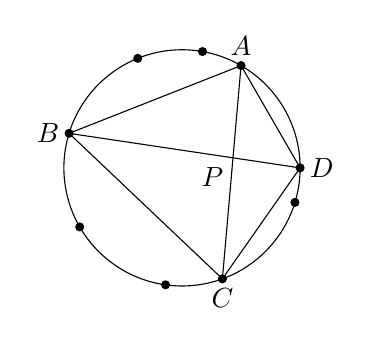
\begin{tikzpicture}
        \draw (0,0) circle (1.5);
        \foreach \i in {0,60,80,112,163,210,262,290,343} {\filldraw (\i:1.5) circle (0.05);};
        \draw (0:1.5) node [right] {$D$} coordinate (D);
        \draw (60:1.5) node [above] {$A$} coordinate (A);
        \draw (163:1.5) node [left] {$B$} coordinate (B);
        \draw (290:1.5) node [below] {$C$} coordinate (C);
        \draw [name path=AC] (A) -- (C);
        \draw [name path=BD] (B) -- (D);
        \draw (A) -- (B) -- (C) -- (D) -- cycle;
        \path [name intersections = {of = AC and BD, by = P}];
        \draw (P) node [below left] {$P$};
    \end{tikzpicture}
\end{center}
解答在这里 设线段$AC$, $BD$在圆内交于点$P$, 连接$AB$, $BC$, $CD$, $DA$, 得到一个四边形, 于是问题转化为$9$个点可组成几个四边形.
所以$N=\mathrm{C}_9^4=126$(个).
\item $5$位女生和$4$位男生彼此身高不一, 现欲选$3$位女生、$2$位男生排成左低右高一行, 有几种排法?
\item 从甲、乙、丙、丁、戊$5$位同学中选$3$位, 安排每一位到京、津、沪旅游中的一地, 有几种选派方法?\\
解答在这里  我们把京, 津, 沪看作$3$个位置, 于是问题就转化为$5$位同学选$3$位分坐$3$个位置的问题, 所以选派方法共有$N=\mathrm{P}_5^3=60$(种).
\item $4$件不同的奖品, 全部奖给$3$位同学, 并要求每人至少一件, 有几种奖励方法?\\
解答在这里 设$4$件奖品为$a$, $b$, $c$, $d$, 显然, 要将它们分成$2, 1, 1$三组, 因此第一步是组合, 得$\mathrm{C}_4^2$; 我们假定$\{a,b\}\{c\}\{d\}$ 是一种组合, 再让它们坐到甲、乙、丙三个位置上去, 因此第二步是排列, 得$\mathrm{P}_3^3$.
所以不同的奖励法共有$N=\mathrm{C}_4^2\mathrm{P}_3^3=36$(种).
\item $5$本不同的理科书和$3$本不同的文科书并排放在书架上, 要求$3$本文科书并列, 有几种不同的放法?
解答在这里  先把$3$本文科书作一个单元与$5$本理科书一起进行全排列, 有$\mathrm{P}_6^6$种排法; 然后考虑$3$本文科书的全排列, 对$\mathrm{P}_3^3$种排法.
根据乘法原理, 共有不同排法为$\mathrm{P}_6^6\mathrm{P}_3^3=4320$(种).
\item 联欢会上要演出$4$个歌唱节目和$3$个舞蹈节目, 如果舞蹈节目不能连排, 有几种排串节目的方法?\\
解答在这里  如图, 先排$4$个歌唱节目, 有$\mathrm{P}_4^4$种排法; 再在图中打$\times$处排入舞蹈节目, 有$\mathrm{P}_5^3$种排法. 因此共有不同排法: $\mathrm{P}_4^4\mathrm{P}_5^3=1440$(种).
\begin{center}
    \begin{tikzpicture}[scale = 0.6]
        \foreach \i in {1,3,...,9} {\draw (\i,0.5) node {$\times$};};
        \foreach \i in {2,4,6,8} {\draw (\i,0.5) node {歌};};
        \draw (0.5,0) -- (9.5,0) (0.5,1) -- (9.5,1);
        \foreach \i in {0.5,1.5,...,9.6} {\draw (\i,0) -- (\i,1);};
    \end{tikzpicture}
\end{center}
\item $5$名运动员参加$100$米决赛, 如果每人到达终点的顺序各不相同, 问: 甲比乙先到达终点的可能有几种?\\
解答在这里 解法一  甲第一个到达, $N_1=\mathrm{P}_4^4$; 甲第二个到达, $N_2=\mathrm{P}_3^1\mathrm{P}_3^3$; 甲第三个到达$N_3=\mathrm{P}_2^1\mathrm{P}_3^3$; 甲第四个到达, $N_4=\mathrm{P}_3^3$.所以$N=\mathrm{P}_4^4+\mathrm{P}_3^1\mathrm{P}_3^3+\mathrm{P}_2^1\mathrm{P}_3^3+\mathrm{P}_3^3=60$(种).
解法二  5名运动员到达终点的顺序有$\mathrm{P}_5^5=120$(种), 而甲先于乙到达和乙先于甲到达的情况是对称出现的.所以$N=\dfrac 12\mathrm{P}_5^5=60$(种).
解法三  $N=\mathrm{C}_5^2\mathrm{P}_3^3=60$(种).
\item 若$x\in \{2,3,7\}$, $y\in \{-31,-20,4\}$, 则$xy$可表示不同的值的个数是\bracket{20}.
\fourch{$1+1=2$}{$1+1+1=3$}{$2\times 3=6$}{$3\times 3=9$}
\item 已知复数$a+b\mathrm{i}$, 其中$a,b\in \{0,1,2,3,4,5,6,7,8,9\}$, 则可组成的不同虚数个数为\bracket{20}.
\fourch{$100$}{$90$}{$81$}{$46$}
\item 如图, 用$4$种不同的颜色涂入图中的矩形$A$, $B$, $C$, $D$中, 要求相邻的矩形涂色不同, 则不同的涂法共有\bracket{20}.
\fourch{$72$种}{$48$种}{$24$种}{$12$种}
\begin{center}
    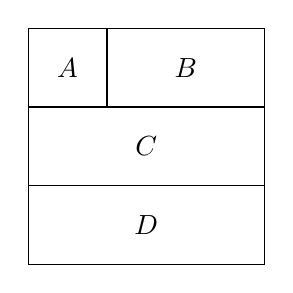
\begin{tikzpicture}
        \draw (0,0) rectangle (3,3);
        \draw (0,1) -- (3,1) (0,2) -- (3,2) (1,2) -- (1,3);
        \draw (1.5,0.5) node {$D$} (1.5,1.5) node {$C$} (0.5,2.5) node {$A$} (2,2.5) node {$B$};
    \end{tikzpicture}
\end{center}
\item 把$10$个苹果分成三堆, 要求每堆至少$1$个, 至多$5$个, 则不同的分法共有\bracket{20}.
\fourch{$4$种}{$5$种}{$6$种}{$7$种}
\item 沿着长方体的棱, 从一个顶点到与它相对的另一个顶点的最近路线共有\bracket{20}.
\fourch{$3$条}{$4$条}{$5$条}{$6$条}
\item 若$a,b\in \mathbf{N}$, 且$a+b\le 6$, 则复数$a+b\mathrm{i}$共有\blank{50}个.
\item 若整数$x,y$满足$|x|<4$, $|y|<5$, 则以$(x,y)$为坐标的点共有\blank{50}个.
\item 如图是一电路图, 从$A$到$B$共有\blank{50}条不同的线路可通电.
\begin{center}
    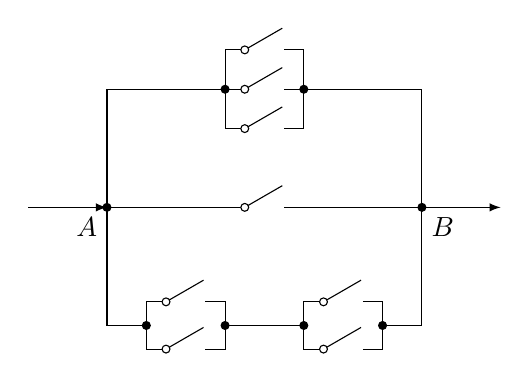
\begin{tikzpicture}[>=latex]
        \draw [->] (-1,0) -- (0,0) node [below left] {$A$};
        \draw [->] (4,0) node [below right] {$B$}-- (5,0); 
        \draw (0,0) -- (0,-1.5) -- (0.5,-1.5) (1.5,-1.5) -- (2.5,-1.5) (3.5,-1.5) -- (4,-1.5) -- (4,0);
        \draw (0,0) -- (0,1.5) -- (1.5,1.5)  (2.5,1.5) -- (4,1.5) -- (4,0);
        \draw (0,0) -- (1.75,0)  (2.25,0) -- (4,0);
        \draw (1.75,0) --++ (30:0.55);
        \filldraw [fill = white, draw = black] (1.75,0) circle (0.05);
        \draw (0.5,-1.5) --++ (0,0.3) --++ (0.25,0) ++ (0.5,0) --++ (0.25,0) --++ (0,-0.3) (0.5,-1.5) --++ (0,-0.3) --++ (0.25,0) ++ (0.5,0) --++ (0.25,0) --++ (0,0.3);
        \draw (2.5,-1.5) --++ (0,0.3) --++ (0.25,0) ++ (0.5,0) --++ (0.25,0) --++ (0,-0.3) (2.5,-1.5) --++ (0,-0.3) --++ (0.25,0) ++ (0.5,0) --++ (0.25,0) --++ (0,0.3);
        \draw (1.5,1.5) --++ (0,0.5) --++ (0.25,0) ++ (0.5,0) --++ (0.25,0) --++ (0,-0.5) (1.5,1.5) --++ (0,-0.5) --++ (0.25,0) ++ (0.5,0) --++ (0.25,0) --++ (0,0.5) (1.5,1.5) --++ (0.25,0) ++ (0.5,0) --++ (0.25,0);
        \draw (0.75,-1.2) --++ (30:0.55);
        \filldraw [fill = white, draw = black] (0.75,-1.2) circle (0.05);
        \draw (0.75,-1.8) --++ (30:0.55);
        \filldraw [fill = white, draw = black] (0.75,-1.8) circle (0.05);
        \draw (2.75,-1.2) --++ (30:0.55);
        \filldraw [fill = white, draw = black] (2.75,-1.2) circle (0.05);
        \draw (2.75,-1.8) --++ (30:0.55);
        \filldraw [fill = white, draw = black] (2.75,-1.8) circle (0.05);
        \draw (1.75,1) --++ (30:0.55);
        \filldraw [fill = white, draw = black] (1.75,1) circle (0.05);
        \draw (1.75,1.5) --++ (30:0.55);
        \filldraw [fill = white, draw = black] (1.75,1.5) circle (0.05);
        \draw (1.75,2) --++ (30:0.55);
        \filldraw [fill = white, draw = black] (1.75,2) circle (0.05);
        \filldraw (0,0) circle (0.05) (4,0) circle (0.05) (1.5,1.5) circle (0.05) (2.5,1.5) circle (0.05) (0.5,-1.5) circle (0.05) (1.5,-1.5) circle (0.05) (2.5,-1.5) circle (0.05) (3.5,-1.5) circle (0.05);
    \end{tikzpicture}
\end{center}
\item 若集合$M=\{-1,1,2\}$, 且$a,b,r\in M$, 则$(x-a)^2+(y-b)^2=r^2$所表示的不同圆共有\blank{50}个.
\item 若$a\in \{-1,2,3\}$, $b\in \{0,3,4,5\}$, $R\in \{1,2\}$, 则方程$(x-a)^2+(y-b)^2=R^2$所表示的不同圆有\blank{50}个.
\item 某乒乓球队行男运动员$7$人, 女运动员$6$人, 从中选出一名担任队长, 共有\blank{50}种不同方案; 从中派出$2$人参加男女混合双打, 共有\blank{50}种不同方案.
\item 若$m\in \{-2,-1,0,1,2,3\}$, $n\in \{-3,-2,-1,0,1,2\}$, 且方程$\dfrac{x^2}m+\dfrac{y^2}n=1$是表示中心在原点的双曲线, 则表示不同的双曲线最多有\blank{50}条.
\item $3$张卡片的正反面分别写有数字$1$和$2$, $3$和$4$, $5$和$6$, 若将$3$张卡片并列, 可得到\blank{50}个不同的三位数($6$不能作$9$用).
\item 从$2, 3, 5, 7$这$4$个数字中, 任取两个分别作为分数的分子与分母.\\
(1) 能得到几个不同的分数?\\
(2) 其中有几个是真分数? 几个是假分数?
\item 在六棱锥各棱所在的$12$条直线中, 异面直线共有\bracket{20}.
\fourch{$12$对}{$24$对}{$36$对}{$48$对}
\item 有一排$5$个信号的显示窗, 每个窗可亮红灯、绿灯或不亮灯, 则共可发出的不同信号有\bracket{20}.
\fourch{$2^5$种}{$5^2$种}{$3^5$种}{$5^3$种}
\item $4$位学生各写一张贺卡, 放在一起, 然后每人从中各取一张, 但不能取自己写的那一张贺卡, 则不同的取法共有\bracket{20}.
\fourch{$9$种}{$12$种}{$16$种}{$24$种}
\item $3$封不同的信, 投入$4$个信箱, 则并有不同的投法\blank{50}种.
\item $4$个学生报名参加跳高, 跳远, 游泳比赛, 每人限报$1$项, 则不同的报名方法共有\blank{50}种.
\item 若集合$A=\{a_1,a_2,a_3,a_4,a_5\}$, $B=\{b_1,b_2,b_3\}$, 则从集合$A$到$B$可建立\blank{50}个不同的映射, 从集合$B$到集合$A$可建立\blank{50}个不同的映射.
\item 如图, 用4种不同的颜色涂入图中编兮为1, 2, 3, 4的正方形, 要求每个正方形只涂一种颜色, 且有公共边的两个正方形颜色不同, 则共有多少种不同的涂法?
\begin{center}
    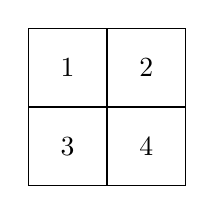
\begin{tikzpicture}
        \draw (0,0) rectangle (2,2);
        \draw (1,0) -- (1,2) (0,1) -- (2,1);
        \draw (0.5,1.5) node {$1$} (1.5,1.5) node {$2$} (0.5,0.5) node {$3$} (1.5,0.5) node {$4$};
    \end{tikzpicture}
\end{center}
\item 从$1$到$100$的自然数中, 每次取两个不同的数相加, 使它们的和不大于$100$, 有几种取法? ($3+6$与$4+5$算作不同的取法).
\item 从$1$到$200$这$200$个自然数中, 各个数位上都不含有数字$8$的数有几个?
\item 有一角硬币$3$枚, 贰元币$6$张, 百元币$4$张, 共可组成多少种不同的币值.
\item 设$a\in \mathbf{N}$, 且$a<27$, 则$(27-a)(28-a)\cdots (34-a)$等于\bracket{20}.
\fourch{$\mathrm{P}_{27-a}^8$}{$\mathrm{P}_{34-a}^{27-a}$}{$\mathrm{P}_{34-a}^7$}{$\mathrm{P}_{34-a}^8$}
\item $6$人站成一排照相, 其中甲、乙、丙三人要站在一起, 且要求乙、丙分别站在甲的两边, 则不同的排法种数为\bracket{20}.
\fourch{12}{24}{48}{144}
\item 记$8$个同学排成一排的排列数为$m$, $8$个同学排成前后两排(前排$3$人, 后排$5$人)的排列数为$n$, 则$m$, $n$的大小关系是\bracket{20}.
\fourch{$m=n$}{$m>n$}{$m<n$}{$n<m<2n$}
\item 用$0, 1, 2, 3$这$4$个数字, 可以组成无重复数字的四位数的个数是\bracket{20}.
\fourch{$6$}{$12$}{$18$}{$24$}
\item $5$辆汽车从停车场分五班开出, 其中甲车必须在乙车之前开出, 则发车方案种数为\bracket{20}.
\fourch{$24$}{$48$}{$60$}{$96$}
\item 若$\mathrm{P}_n^3=n\mathrm{P}_3^3$, 则$n=$\blank{50}.
\item 若$\mathrm{P}_n^n+\mathrm{P}_{n-1}^{n-1}=x\mathrm{P}_{n+1}^{n+1}$, 则$x=$\blank{50}.
\item 若$\mathrm{P}_{56}^{n+6}:\mathrm{P}_{54}^{n+3}=30800$, 则$n=$\blank{50}.
\item 在$10$只不同的抽屉中, 放入$10$种不同的产品, 每只抽屉只放一种, 共有\blank{50}种不同的放法.
\item 有黄、红、蓝、白、黑五面不同颜色的信号旗, 按不同顺序从左到右排成一排表示不同的信号, 则可表示\blank{50}种不同的信号.
\item $7$位同学站成一排, 按下列要求各存多少种不同的排法:\\
(1) 甲站某一固定位置;\\
(2) 甲站中间, 乙与甲相邻;\\
(3) 甲、乙相邻;\\
(4) 甲、乙两人不能相邻;\\
(5) 甲、乙、丙三人相邻;\\
(6) 甲、乙两人不站在排头和排尾;\\
(7) 甲、乙、丙三人中任何两人都不相邻;\\
(8) 甲、乙两人必须相邻, 且丙不站在排头和排尾.
\item 在由$0, 1, 2, 3, 4, 5$这$6$个数字组成的无重复数字的六位数中, 个位数字小于十位数字的个数是\bracket{20}.
\fourch{$210$}{$300$}{$464$}{$600$}
\item 在由数字$1$, $2$, $3$, $4$, $5$组成数字不重复的五位数中, 小于$50000$的偶数有\bracket{20}.
\fourch{$60$个}{$48$个}{$36$个}{$24$个}
\item 由$0$, $1$, $2$, $3$, $4$, $5$这$6$个数字组成数字不重复且大于$345012$的六位数的个数是\bracket{20}.
\fourch{$360$}{$270$}{$269$}{$245$}
\item $6$个停车位置, 有$3$辆汽车需要停放, 若要使$3$个空位连在一起, 则停放方法数为\bracket{20}.
\fourch{$\mathrm{P}_4^4$}{$\mathrm{P}_6^3$}{$\mathrm{P}_6^4$}{$\mathrm{P}_3^3$}
\item $6$张同排连号的电影票, 分给$3$名教师和$3$名学生, 若要求师生相间而坐, 则不同的分法数为\bracket{20}.
\fourch{$\mathrm{P}_3^3\mathrm{P}_4^3$}{$(\mathrm{P}_3^3)^2$}{$2(\mathrm{P}_3^3)^2$}{$\mathrm{P}_6^6-(\mathrm{P}_3^3)^2$}
\item 取$1, 2, 3, 4, 5$这$5$个数字中的两个分别作为一个对数的底数和真数, 则所得的不同值有\bracket{20}.
\fourch{$12$个}{$13$个}{$16$个}{$20$个}
\item 由$0, 1, 2, 3, 4, 5$这$6$个数字组成的无重复数字的三位数中, 奇数个数与偶数个数之比为\bracket{20}.
\fourch{$1:1$}{$2:3$}{$12:13$}{$21:23$}
\item 直线$Ax+By=0$的系数$A$, $B$可以在$0, 1, 2, 3, 5, 7$这六个数字中取值, 则这些方程所表示的不同直线有\bracket{20}.
\fourch{$30$条}{$23$条}{$22$条}{$14$条}
\item 已知集合$M=\{a_1,a_2,a_3\}$, $P=\{b_1,b_2,b_3,b_4,b_5,b_6\}$, 若$M$中的不同元素对应到$P$中的不同像, 则这样的映射个数共有\bracket{20}.
\fourch{$3$}{$20$}{$64$}{$120$}
\item 从$1, 2, \cdots, 10$这$10$个自然数中, 每次取出不同的两个, 使它们的乘积是6的倍数, 则不同的取法总数为\bracket{20}.
\fourch{$14$}{$15$}{$16$}{$17$}
\item 赛前将$4$对乒乓球双打选手介绍给观众, 每对选手要连着介绍, 则介绍这$8$位选手的不同顺序共有\bracket{20}.
\fourch{$\mathrm{P}_8^8$种}{$\mathrm{P}_4^4$种}{$2\mathrm{P}_4^4$种}{$16\mathrm{P}_4^4$种}
\item 要排一张有$5$个独唱节目和$3$个合唱节目的演出节目表, 若合唱节目不排在节目表的第一位置上, 并且任何两个合唱节目不相邻, 则不同的排法总数是\bracket{20}.
\fourch{$\mathrm{P}_8^8$}{$\mathrm{P}_5^5\mathrm{P}_3^3$}{$\mathrm{P}_5^5\mathrm{P}_5^3$}{$\mathrm{P}_3^3\mathrm{P}_5^3$}
\item 由$1, 4, 5,x$这四个数字组成无重复数字的四位数, 若所有$4$位数的各位数字之和为$288$, 则$x$等于\bracket{20}.
\fourch{$2$}{$3$}{$6$}{$8$}
\item $6$个人排成一排, 要求甲、乙、丙$3$人都不排在两端, 求不同排法的种数.
\item $5$男$2$女站成一排, 要求女生不能排在两端, 且又要相邻, 求不同排法的种数.
\item $5$人排成一行, 要求甲、乙$2$人之间至少有$1$人, 求不同排法的种数.
\item $6$人排成一排, 要求甲、乙$2$人之间必有$2$人, 求不同排法的种数.
\item 一排$6$张椅子上坐$3$个人, 每$2$人之间有$1$张空椅子, 求不同排法的种数.
\item $8$张椅子排成一排, 有$4$人就坐, 每人一个座位, 其中恰有$3$个连续空位, 求不同排法的种数.
\item $8$名学生站成前、后两排, 每排$4$人, 其中要求甲、乙$2$人在后排, 丙在前排, 求不同排法的种数.
\item $8$人站成一列纵队, 要求甲、乙、丙$3$人不在排头且要互相隔开, 求不同排法的种数.
\item $8$位同学, 其中有$3$位是三好学生, 他们和班主任合影, 要求班主任坐中间, 而且左、右两边都要有三好学生, 求不同排法的种数.
\item $6$人并排拍照, 要求甲不坐在最左边, 乙不坐在最右边, 求不同排法的种数.
\item 晚会上有$5$个不同的歌唱节目和$3$个不同的舞蹈节目, 分别按以下要求, 各可排出几种不同的节目单:
(1) 前$4$个节目中既要有歌唱节目, 又要有舞蹈节目;\\
(2) $3$个舞蹈节目排在一起;\\
(3) $3$个舞蹈节目彼此隔开;\\
(4) $3$个舞蹈节目先后顺序一定.
\item $6$人划船, 其中$2$人只能划右桨, $1$人只能划左桨, 若要求左、右边各$3$人, 则有几种不同的划法?
\item 个位和百位的数字是奇数, 十位和千位的数字是偶数, 且无重复数字的四位数共有多少个?
\item 星期一上午某教师要上$3$个班级的课, 每班$1$节, 若上午规定限排$4$节课, 且要求$3$节课不能连排, 则这天上午该教师的课程表有几种不同的排法?
\item 某天的课程表排入政治、语文、数学、外语、劳技、体育$6$门课, $1$门课排$1$节, 若第$1$节不能排体育, 第$6$节不能排数学, 则共有几种不同排法?
\item 由$0, 2, 5, 7, 9$这$5$个数字可组成多少个数字不重复且能被$3$整除的四位数?
\item 由$0, 1, 2, 3, 4, 5$这$6$个数字可组成多少个数字不重复且能被$4$整除的四位数? 可组成数字不重复且能被25整除的四位数又有多少?
\item 由$1, 2, 3, 4, 5, 6$这$6$个数字可组成多少个数字不重复且是$6$的倍数的五位数?
\item 由数字$1,2, 3, 4, 5$可以组成没有重复数字的五位数$120$个, 若把这些数从小到大排成一列数: $12345, 12354, \cdots,54321$, 问:\\
(1) $43251$是这一列数的第几个数?\\
(2) 这列数中的第$93$个数是怎样的一个五位数?\\
(3) 求这一列数各数之和(不必具体算出).
\item 用$1, 2, 3, 4, 5, 6$这$6$个数字组成无重复数字的四位数.\\
(1) 奇数数字必须在奇数位的有多少个?\\
(2) 奇数位只排奇数数字的有多少个?\\
(3) 奇数数字不排在奇数位的有多少个?
\item 从$1, 2, 3, 4, 5$这$5$个数字中每次取出$3$个数字组成没有重复数字的三位数, 求所有三位数的个位数的和.
\item 用$1, 7, 8, 9$这$4$个数字组成的四位数中, 分别求所有四位数的各位数字的和与所有四位数的和.
\item 由$1, 4, 5, x$这$4$个不同数字组成数字不重复的四位数, 若所有四位数的数字之和是$180$, 求$x$.
\item 用$0, 1, 2, 3, 4, 5$这$6$个数字组成无重复数字的三位数, 求所有这些三位数之和.
\item 从$1, 2, 3, 4, 8$这$5$个数字中, 任选两个分别作$a^b$中的底数和指数, 则得到的不同值的幂有多少个?
\item 从$1, 2, 3, \cdots, 9$这$9$个数字中任取两个不同的数, 分别作一个对数的真数和底数, 一共可以得到几个不同的对数值? 其中比$1$大的有几个?
\item 若$n\ne m$, 则组合数$\mathrm{C}_n^m$等于\bracket{20}.
\fourch{$\dfrac{\mathrm{P}_n^m}{n!}$}{$\dfrac nm\mathrm{C}_{n-1}^m$}{$\mathrm{C}_m^{n-m+1}$}{$\dfrac n{n-m}\mathrm{C}_{n-1}^m$}
\item 计算$\mathrm{C}_{10}^{r+1}+\mathrm{C}_{10}^{17-r}$, 值不相同的有\bracket{20}.
\fourch{$1$个}{$2$个}{$3$个}{$4$个}
\item 一组$6$条平行线与另一组$3$条平行线互相垂直, 则由它们所围成的矩形个数是\bracket{20}.
\fourch{$16$个}{$45$个}{$24$个}{$90$个}
\item 从$1, 3, 5, 7, 9$这$5$个数字中任取$3$个, 从$2, 4, 6, 8$这$4$个数字中任取$2$个, 组成数字不重复的五位数的个数是\bracket{20}.
\fourch{$\mathrm{P}_5^3\mathrm{P}_4^2$}{$\mathrm{C}_5^3\mathrm{P}_5^3\mathrm{C}_5^2\mathrm{P}_4^2$}{$\mathrm{C}_5^3\mathrm{C}_4^2\mathrm{P}_5^5$}{$\mathrm{P}_5^3\mathrm{P}_6^2$}
\item 从$4$台$A$型和$5$台$B$型的电视机中, 任取$3$台, 要求至少有$A$型和$B$型各一台的取法数为\bracket{20}.
\fourch{$70$}{$140$}{$84$}{$35$}
\item 以正方形的$4$个顶点, $4$边中点和中心这$9$个点中的$3$点为顶点的三角形的个数是\bracket{20}.
\fourch{$84$}{$81$}{$76$}{$73$}
\item 平面内有$9$个点, 其中有$4$个点在一条直线上, 此外无$3$点共线, 经过其中的每$2$个点作直线, 不同直线的条数是\bracket{20}.
\fourch{$31$}{$30$}{$29$}{$28$}
\item 从集合$P=\{1,2,3\}$, $Q=\{1,4,5,6\}$这两个集合中各取一个元素作为平面直角坐标系中点的坐标, 能确定的不同点的个数是\bracket{20}.
\fourch{$11$}{$12$}{$23$}{$24$}
\item 计算: $\mathrm{C}_m^5-\mathrm{C}_{m+1}^5+\mathrm{C}_m^4=$\blank{50}.
\item 计算: $\mathrm{C}_{96}^{94}+\mathrm{C}_{97}^{95}+\mathrm{C}_{98}^{96}+\mathrm{C}_{99}^{97}=$\blank{50}.
\item 计算: $\mathrm{C}_2^2+\mathrm{C}_3^2+\mathrm{C}_4^2+\cdots +\mathrm{C}_{10}^2=$\blank{50}.
\item 计算: $\mathrm{C}_3^0+\mathrm{C}_4^1+\mathrm{C}_5^2+\mathrm{C}_6^3+\cdots +\mathrm{C}_{20}^{17}=$\blank{50}.
\item 从$5$名学生中任选$3$名学生分别担任3种不同的职务, 共有\blank{50}种小同的办法.
\item 有$3$名学生分别担任$5$种不同职务中的$3$个不同职务, 共有\blank{50}种不同分法.
\item 在两条异面直线上分别各有$5$个点和$4$个点, 每两点确定一条直线, 一共有\blank{50}条直线.
\item 直线$l_1\parallel l_2$, $l_1$上有$4$个点, $l_2$上有$6$个点, 以这些点为端点连接成线段, 则它们在$l_1$与$l_2$之间的交点最多有\blank{50}个.
\item $M$和$N$是两个不重合的平面, 在平面$M$内取$5$个点, 在平面$N$内取$4$个点, 则由这些点最多能决定不同位置的三棱锥有\blank{50}个.
\item 平面内共有$17$个点, 其中有且仅有$5$个点共线, 以这些点中的$3$个点为顶点的三角形共有\blank{50}个.
\item 以三棱柱的顶点为顶点的四面体的个数为\blank{50}.
\item 平面内有$7$条不同的直线, 其中有且仅有两条直线互相平行, 则这$7$条直线最多能围成的三角形有\blank{50}个.
\item 已知一些点的坐标$(x,y)$满足$|x|<2$, $|y|<2$且$x\in \mathbf{Z}$, $y\in \mathbf{Z}$, 若以这些点的其中三点为顶点作三角形, 则这样的三角形共有\bracket{20}.
\fourch{$72$个}{$76$个}{$80$个}{$84$个}
\item 以正方体的顶点为顶点的四而体个数是\bracket{20}.
\fourch{$70$}{$64$}{$58$}{$24$}
\item 有甲、乙、丙$3$项任务, 其中甲需$2$人承担, 乙、丙各需$1$人承担, 现从$10$人中选派$4$人承担这$3$项任务, 则不同的选法数共有\bracket{20}.
\fourch{$1260$种}{$2025$种}{$2520$种}{$5040$种}
\item 将$5$名学生分配到$4$个不同的科技小组参加活动, 要求每个科技小组至少有一名学生参加, 则不同的分配方法共有\bracket{20}.
\fourch{$60$种}{$120$种}{$240$种}{$480$种}
\item 将$4$名教师分配到$3$个班级去参加活动, 要求每班至少$1$名的分配方法有\bracket{20}.
\fourch{$72$种}{$48$种}{$36$种}{$24$种}
\item 高三年级有$8$个班, 分派$4$个数学教师任教, 每个教师教两个班, 则不同的分派方法有\bracket{20}.
\fourch{$\mathrm{P}_8^2\mathrm{P}_6^2\mathrm{P}_4^2\mathrm{P}_2^2$种}{$\mathrm{C}_8^2\mathrm{C}_6^2\mathrm{C}_4^2\mathrm{C}_2^2$种}{$\mathrm{C}_8^2\mathrm{C}_6^2\mathrm{C}_4^2\mathrm{C}_2^2\mathrm{C}_4^4$种}{$\dfrac{\mathrm{C}_8^2\mathrm{C}_6^2\mathrm{C}_4^2\mathrm{C}_2^2}{4!}$种}
\item 现有男、女学生共$8$人, 从男生中选$2$人, 从女生中选$1$人分别参加数学、物理与化学三科竞赛, 共有$90$种不同的选派方案, 则男、女生人数为\bracket{20}.
\fourch{男生$2$人, 女生$6$人}{男生$3$人, 女生$5$人}{男生$5$人, 女生$3$人}{男生$6$人, 女生$2$人}
\item 把字母$a$, $a$, $a$, $a$, $b$, $b$, $b$排成一列, 其中任何两个$b$不能相邻的排法共有\bracket{20}.
\fourch{$4$种}{$10$种}{$24$种}{$60$种}
\item 已知$a\in \{-2,-1,0,1,2,3,4\}$, $b\in \{-3,-2,-1,0,1,2,3,4,5\}$, 则方程$\dfrac{x^2}a+\dfrac{y^2}b=1$表示的不同双曲线条数最多是\bracket{20}.
\fourch{$48$}{$26$}{$22$}{$14$}
\item 若$m$, $n$是不大于$6$的非负整数, 则$\mathrm{C}_6^mx^2+\mathrm{C}_6^ny^2=1$表示不同的椭圆个数是\bracket{20}.
\fourch{$42$}{$30$}{$12$}{$6$}
\item 从$5$个学校中选出$8$名学生组成代表团, 要求每校至少有$1$人的选法种数是\bracket{20}.
\fourch{$\mathrm{C}_5^1+\mathrm{C}_5^1\mathrm{C}_4^1+\mathrm{C}_5^1\mathrm{C}_4^1\mathrm{C}_3^1$}{$\mathrm{C}_5^3+\mathrm{C}_5^2\mathrm{C}_4^1+\mathrm{C}_5^1\mathrm{C}_4^1\mathrm{C}_3^1$}{$\mathrm{C}_5^1+\mathrm{P}_5^2+\mathrm{C}_5^3$}{$\mathrm{C}_8^5$}
\item 空间有$n$个点, 任意$4$点均不共面, 连接其中任意两点均有一直线, 则成为异面直线的对数为\bracket{20}.
\fourch{$\mathrm{C}_n^4$}{$2\mathrm{C}_n^4$}{$3\mathrm{C}_n^4$}{$\mathrm{P}_n^4$}
\item 若$\mathrm{C}_7^x=\mathrm{C}_7^2$, 则$x=$\blank{50}.
\item 若$\mathrm{C}_{18}^{2x}=\mathrm{C}_{18}^{16-x}$, 则$x=$\blank{50}.
\item 若$\mathrm{C}_x^{12}=\mathrm{C}_x^8$, 则$x=$\blank{50}.
\item 若$\mathrm{C}_x^3:\mathrm{C}_x^2=44:3$, 则$x=$\blank{50}.
\item 若$3\mathrm{C}_{x-3}^{x-7}=5\mathrm{P}_{x-4}^2$, 则$x=$\blank{50}.
\item 若$\mathrm{C}_{17}^{2x}+\mathrm{C}_{17}^{2x-1}=\mathrm{C}_{18}^6$, 则$x=$\blank{50}.
\item 异面直线$l_1$和$l_2$分别有$m$个和$n$($m,n\ge 3$)个不同的点, 若以这些点为顶点, 可构成\blank{50}个三角形, \blank{50}个四面体.
\item 一条直线$a$上有$n$个点, 平面$\alpha$内有$m$个点, 以这些点为顶点, 最多可确定\blank{50}个三棱锥.
\item 有两个同心圆, 在外圆周上有相异的$6$个点, 内圆周上有相异的$3$个点, 由这$9$个点所确定的直线最多有\blank{50}条, 最少有\blank{50}条.
\item 已知$\angle AOB$的一边$OA$上有不同的$8$个点, 在另一边$OB$上有不同的$3$个点, 现从$OA$, $OB$上分别取一点作连线, 则由这些直线相交的交点在$\angle AOB$内的个数最多有\blank{50}个.
\item 解不等式: $\dfrac 13<\dfrac{\mathrm{C}_{x+1}^3}{\mathrm{C}_{x-1}^1}<7$.
\item 解不等式: $\mathrm{C}_n^{n-5}>\mathrm{C}_{n-2}^3+2\mathrm{C}_{n-2}^2+n-2$.
\item 解不等式: $\mathrm{C}_{21}^{x-4}<\mathrm{C}_{21}^{x-2}<\mathrm{C}_{21}^{x-1}$.
\item 解不等式: $\mathrm{C}_k^0+\mathrm{C}_k^1+2\mathrm{C}_k^2+3\mathrm{C}_k^3+\cdots +k\mathrm{C}_k^k<500$.
\item 解方程: $\mathrm{C}_{16}^{x^2-x}=\mathrm{C}_{16}^{5x-5}$.
\item 解方程: $\mathrm{C}_{x+3}^{x+1}=\mathrm{C}_{x+1}^{x-1}+\mathrm{C}_{x+1}^x+\mathrm{C}_x^{x-2}$.
\item 计算: $\mathrm{C}_{2n}^{17-n}+\mathrm{C}_{13+n}^{3n}$.
\item 计算: $\mathrm{C}_{3n}^{38-n}+\mathrm{C}_{21+n}^{3n}$.
\item 化简: $1\cdot 1!+2\cdot 2!+\cdots +10\cdot 10!$.
\item 求证: $\dfrac 1{k!}-\dfrac 1{(k+1)!}=\dfrac k{(k+1)!}$.
\item 化简: $\dfrac 1{2!}+\dfrac 2{3!}+\cdots +\dfrac n{(n+1)!}$.
\item 求证: $\dfrac{k+2}{k!+(k+1)!+(k+2)!}=\dfrac 1{(k+1)!}-\dfrac 1{(k+2)!}$.
\item 求和: ; $\dfrac 3{1!+2!+3!}+\dfrac 4{2!+3!+4!}+\cdots +\dfrac{n+2}{n!+(n+1)!+(n+2)!}$.
\item 求证: $\mathrm{C}_n^k=\mathrm{C}_2^0\mathrm{C}_{n-2}^k+\mathrm{C}_2^1\mathrm{C}_{n-2}^{k-1}+\mathrm{C}_2^2\mathrm{C}_{n-2}^{k-2}$($k\ge 2$).
\item 求证: $n!+\dfrac{(n+1)!}{1!}+\dfrac{(n+2)!}{2!}+\cdots +\dfrac{(n+m)!}{m!}=n!\mathrm{C}_{n+m+1}^{n+1}$.
\item $n$个不同的球放入$n$个不同的盒子中, 若恰好有一个盒子是空盒, 则共有几种不同的放法?
\item 从集合$M=\{1,2,3,4,5\}$到集合$N=\{a,b,c\}$的映射, 要求集合$N$中的元素在集合$M$中都有原像, 这样的映射有几种?
\item 如图, $A,B,C\in l_1$, $D,E,F,G\in l_2$, $H$不属于$l_1\cup l_2$, 以这$8$个点中的$3$个点为顶点, 最多可作多少个不同的三角形?
\begin{center}
    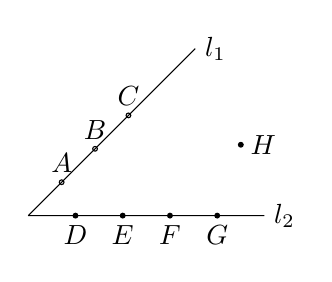
\begin{tikzpicture}[scale = 0.6]
        \draw (0,0) -- (5,0) (0,0) -- (45:5);
        \filldraw (1,0) circle (0.05) node [below] {$D$} (2,0) circle (0.05) node [below] {$E$} (3,0) circle (0.05) node [below] {$F$} (4,0) circle (0.05) node [below] {$G$} (4.5,1.5) circle (0.05) node [right] {$H$};
        \draw (45:1) circle (0.05) node [above] {$A$} (45:2) circle (0.05) node [above] {$B$} (45:3) circle (0.05) node [above] {$C$};
        \draw (5,0) node [right] {$l_2$} (45:5) node [right] {$l_1$};
    \end{tikzpicture}
\end{center}
\item $\angle AOB$的两边$OA$, $OB$上分别有异于顶点$O$的$5$个点和$6$个点, 这$12$个点(连同$O$点)可作几条不同直线和几个不同的三角形?
\item 在$ABCD$中, $M$, $N$是边$AB$的三等分点, $P$是边$CD$的中点, 从$A$, $B$, $C$, $D$, $M$, $N$, $P$这$7$个点中选$3$个作为三角形的顶点, 一共可以构成几个不同的三角形? 其中面积最小的三角形有几个?
\item 以四棱台的顶点为顶点, 时组成多少个四面体?
\item 正方体有$8$个顶点, 每$3$点确定$1$个平面, 一共可确定多少个平面?
\item 从集合$\{51,52,53,\cdots ,99\}$中任选$2$个数, 使这$2$个数的和为偶数, 有多少种不同的选法?
\item 从$1$到$100$的自然数中, 每次取两个不同的数相加, 使它们的和不大于$100$, 有几种不同的取法($1+4$与$2+3$算不同的取法, $2+3$与$3+2$算相同的取法)?
\item 从$1$到$18$这$18$个自然数中任选$3$个, 使它们的和是$3$的倍数, 有几种选法?
\item 从$5$个男乒乓球运动员和$4$个女乒乓球运动员中选出$2$男、$2$女进行乒乓球混合双打, 有多少种不同的分组方法?
\item 有编号为$1, 2, 3, 4, 5, 6, 7$的$7$个球和编号为$1, 2, 3, 4, 5, 6, 7$的$7$只盒子, 将这$7$个球放入这$7$只盒子中, 要求每只盒子放$1$个, 恰使其中$4$个球的编号与盒子的编号相同, 一共有多少种不同的投放方法?
\item $9$件相同的奖品分给$3$个学生, 每人至少分得$2$件奖品, 一共存几种不同的分法?
\item $7$个相同的球任意放入$4$个不同的盒子中, 每个盒子至少有$1$个球的不同放法有几种?
\item 在连续的$6$次射击中, 恰好命中$4$次的情形有多少种?
\item 在所有的三位数中(数字允许重复), 百位数字, 十位数字, 个位数字依次减小的有多少个? 仅是个位数字比百位数字小的有多少个?
\item 圆上有$10$个点, 每两点连成一条线段, 这些线段在圆内最多有多少个交点?
\item 将分别写有$a,b,c,d,e,1,2,3,4,5$的$10$张纸片排成一列, 要求$5$在最前, $1$在最后, 且数字从大到小, 字母按英文字母表的先后顺序排列, 则有多少种不同的排法?
\item 从$1, 2,\cdots, 10$这$10$个数中任取$3$个互不相邻的自然数, 有儿种不同的取法?
\item 从$6$个运动员中, 选出$4$人参加$4\times 100$米接力赛跑, 若其中甲、乙两人都不能跑第一棒, 共有多少种参赛方案?
\item 从$7$名运动员中, 选出$4$人参加$4\times 100$米接力赛跑, 若要求甲、乙两人都不跑中间两棒, 共有多少种参赛方案?
\item 有$6$名运动员参加$4\times 100$米接力跑, 其中甲不能跑第一棒, 乙不跑第四棒, 共有多少种参赛的方法?
\item $3$天中, 考政治、语文、外语、数学、物理和化学$6$科.\\
(1)每天考一文一理, 有几种不同的安排方法?\\
(2)每天考一文一理, 且语文、数学不能同一天考, 有几种不同的安排方法?
\item 在无重复数字的四位数中, 其中恰有$2$个奇数数字和$2$个偶数数字的四位数共有多少个?
\item 从$1, 3, 5, 7$这$4$个数字中任取$3$个, 从$0, 2, 4$这$3$个数字中任取$2$个, 共可组成多少个无重复数字的五位数?
\item $10$个人分乘$3$辆汽车, 要求甲车坐$5$人, 乙车坐$3$人, 丙车坐$2$人, 有多少种不同的乘车方法?
\item 某市今年有$8$项重点工程需要建设, 由甲、乙、丙、丁$4$个建筑公司承包, 若要求甲承包$3$项, 乙承包$1$项, 丙、丁各承包$2$项, 则共有多少种不同的承包方案?
\item 有$6$本不同的书, 分给甲、乙、丙$3$人, 按下列要求, 各有几种不同的分法:\\
(1) 甲得$1$本, 乙得$2$本, 丙得$3$本;\\
(2) 每人$2$本;\\
(3) $1$人$1$本, $1$人$2$本, $1$人$3$本.
\item 已知集合$A$和集合$B$各含有$12$个元素, $A\cap B$含有$4$个元素, 试求同时满足下列两个条件的集合$C$的个数:\\
(1) $C\subset (A\cup B)$, 且$C$中含有$3$个元素;\\
(2) $C\cap A\ne \varnothing$.
\item 有翻译$8$人, 其中$3$人只会英语, $2$人只会日语, 其余$3$人既会英语又会日语, 现从中选$6$人, 安排$3$人翻译英语, $3$人翻译日语, 则不同的安排方法有多少种?
\item 求二项式$(2x-\dfrac 3{2x^2})^7$展开式的第四项的二项式系数和笫四项的系数.\\
解答在这里  因为$T_4=T_{3+1}=\mathrm{C}_7^3(2x)^{7-3}(-\dfrac 32x^{-2})^3=\mathrm{C}_7^32^4(-\dfrac 32)^3x^{-2}$,
所以第四项的二项式系数为$\mathrm{C}_7^3$, 即$35$; 第四项的系数为$\mathrm{C}_7^3\cdot 2^4(-\dfrac 32)^3$, 即$-1890$.
\item 求$(1+x)+(1+x)^2+(1+x)^3+\cdots +(1+x)^{2n}$($n\in \mathbf{N}$)的展开式中念$x^n$项的系数.\\
解答在这里 解法一  考虑$(1+x)^k$($n\le k\le 2n$)展开式的通项, 在$T_{r+1}=\mathrm{C}_k^rx^r$中, 令$r=n$, 得$T_{n-1}=\mathrm{C}_k^nx^n$, 故$x^n$项的系数为
\begin{align*} \mathrm{C}_n^n+\mathrm{C}_{n+1}^n+\mathrm{C}_{n+2}^n+\cdots +\mathrm{C}_{2n}^n&=\mathrm{C}_{n+1}^{n+1}+\mathrm{C}_{n+1}^n+\mathrm{C}_{n+2}^n+\cdots +\mathrm{C}_{2n}^n\\
&=\mathrm{C}_{n+2}^{n+1}+\mathrm{C}_{n+2}^n+\cdots +\mathrm{C}_{2n}^n \\ &=\cdots =\mathrm{C}_{2n}^{n+1}+\mathrm{C}_{2n}^n \\ &=\mathrm{C}_{2n+1}^{n+1}.
\end{align*}
解法二  题中的多项式是以$(1+x)$为公比、项数为$2n$的等比数列的和, 于是, 当$x\ne 0$时, 原式$=\dfrac{(1+x)[(1+x)^{2n}-1]}{(1+x)-1}=\dfrac{(1+x)^{2n+1}-(1+x)}x$.
因此, 只需求$(1+x)^{2n+1}$的展开式中含$x^{n+1}$项的系数即可.
而$(1+x)^{2n+1}$展开式的通项为$T_{r+1}=\mathrm{C}_{2n+1}^rx^r$, 令$r=n+1$, 得$T_{n+2}=\mathrm{C}_{2n-1}^{n+1}x^{n+1}$
所以题中含$x^n$项的系数为$\mathrm{C}_{2n-1}^{n+1}$.
\item 在$(\sqrt x+\dfrac 1{\sqrt[3]x})^{100}$的展开式中, 有多少项是有理项?\\
解答在这里  考虑$(x^{\frac 12}+x^{-\frac 13})^{100}$展开式的通项$T_{r+1}=\mathrm{C}_{100}^rx^{\frac{100-r}2}\cdot (x^{-\frac 13})^r=\mathrm{C}_{100}^rx^{50-\dfrac{3r}6}$.
令$r=6k$($k\in \mathbf{Z}$), 则$0\le 6k\le 100$, 即$r=0,6,12,\cdots ,96$.
因此共有$17$个有理项.
\item 求$(x^2+\dfrac 1{x^2}-2)^3$展开式中含$x^2$项的表达式.\\
解答在这里  原式$=(x-\dfrac 1x)^6$, 它的展开式的通项为$T_{r+1}=\mathrm{C}_6^rx^{6-r}(-x^{-1})^r=(-1)^r\mathrm{C}_6^rx^{6-2r}$.
令$r=2$, 得$T_{2+1}=\mathrm{C}_6^2x^2=15x^2$, 所以含$x^2$的项为$15x^2$.
\item 求$(1+x+x^2)(1-x)^{10}$展开式中含$x^4$项的系数.\\
解答在这里 原式$=(1-x^3)(1-x)^9$.
$(1-x)^9$展开式的通项为$T_{r+1}=\mathrm{C}_9^r(-x)^r$.
令$r=4$, 得$T_{4+1}=\mathrm{C}_9^4x^4$.令$r=1$, 得$T_{1+1}=-\mathrm{C}_9^1x$.
故$x^4$的系数为$\mathrm{C}_9^4+\mathrm{C}_9^1=135$.
\item 求$(ax+by+cz)^n$的展开式中含$x^py^qz^r$项的系数, 其中$p+q+r=n$($p,q,r,n\in \mathbf{N}$).
解答在这里  原式$=[(ax+by)+cz]^n$, 其展开式的通项为$T_{k+1}=\mathrm{C}_n^k(ax+by)^{n-k}\cdot (cz)^k$.
令$k=r$, 得$T_{r+1}=\mathrm{C}_n^r(ax+by)^{n-r}\cdot (cz)^r$.
而$(ax+by)^{n-r}$展开式的通项为$T'_{s+1}=\mathrm{C}_{n-r}^s(ax)^{n-r-s}\cdot (by)^s$.
令$s=q$, 得$T'_{q+1}=\mathrm{C}_{n-r}^q(ax)^{n-r-q}\cdot (by)^q=\mathrm{C}_{n-r}^q(ax)^p\cdot (by)^q$.
故$x^py^qz^r$的系数为$\mathrm{C}_n^r\cdot \mathrm{C}_{n-r}^qa^pb^qc^r$.
\item 求$(x+\dfrac 1x-1)^5$展开式中的常数项.\\
解答在这里  把$[(x+\dfrac 1x)-1]^5$直接展开,
即$[(x+\dfrac 1x)-1]^5=(x+\dfrac 1x)^5-5(x+\dfrac 1x)^4+10(x+\dfrac 1x)^3-10(x+\dfrac 1x)^2+5(x+\dfrac 1x)-1$.
考虑$x+\dfrac 1x$的对称性, 只打在它的偶次幂中, 其展开式才会出现常数项.
所以常数项为$(-5)\times 6+(-10)\times 2-1=-51$.
\item 求证: $4^n-4^{n-1}\mathrm{C}_n^1+4^{n-2}\mathrm{C}_n^2-4^{n-3}\mathrm{C}_n^3+\cdots +4(-1)^{n-1}\mathrm{C}_n^{n-1}+(-1)^n\mathrm{C}_n^n=3^n$($n\in \mathbf{N}$).\\
解答在这里  在``$(a+b)^n=\mathrm{C}_n^0a^n+\mathrm{C}_n^1a^{n-1}b+\cdots +\mathrm{C}_n^nb^n$''中, 令$a=4$, $b=-1$得
$4^n-4^{n-1}\mathrm{C}_n^1+4^{n-2}\mathrm{C}_n^2-4^{n-3}\mathrm{C}_n^3+\cdots +4\times (-1)^{n-1}\mathrm{C}_n^{n-1}+(-1)^n\mathrm{C}_n^n=(4-1)^n=3^n$($n\in \mathbf{N}$).
\item 求证: $1-\mathrm{C}_n^2+\mathrm{C}_n^4-\mathrm{C}_n^6+\mathrm{C}_n^8-\mathrm{C}_n^{10}+\cdots =(\sqrt 2)^n\cos \dfrac{n\pi }4$,
$\mathrm{C}_n^1-\mathrm{C}_n^3+\mathrm{C}_n^5-\mathrm{C}_n^7+\mathrm{C}_n^9-\mathrm{C}_n^{11}+\cdots =(\sqrt 2)^n\sin \dfrac{n\pi }4$.\\
解答在这里  在$(a+b)^n=\mathrm{C}_n^0a^n+\mathrm{C}_n^1a^{n-1}b+\cdots +\mathrm{C}_n^{n-1}ab^{n-1}+\mathrm{C}_n^nb^n$中, 令$a=1$, $b=\mathrm{i}$, 则
\begin{align*} 
(1+\mathrm{i})^n=&\mathrm{C}_n^0+\mathrm{C}_n^1\mathrm{i}+\mathrm{C}_n^2\mathrm{i}^2+\mathrm{C}_n^3\mathrm{i}^3+\mathrm{C}_n^4\mathrm{i}^4+\cdots +\mathrm{C}_n^n\mathrm{i}^n \\ &=(\mathrm{C}_n^0-\mathrm{C}_n^2+\mathrm{C}_n^4-\mathrm{C}_n^6+\mathrm{C}_n^8-\mathrm{C}_n^{10}+\cdots)+(\mathrm{C}_n^1-\mathrm{C}_n^3+\mathrm{C}_n^5-\mathrm{C}_n^7+\mathrm{C}_n^9-\mathrm{C}_n^{11}+\cdots)\mathrm{i}
\end{align*}
又$(1+i)^n=[\sqrt 2(\cos \dfrac{\pi }4+i\sin \dfrac{\pi }4)]^n=(\sqrt 2)^n(\cos \dfrac{n\pi }4+i\sin \dfrac{n\pi }4)$.
比较上述两式, 即得欲证.
\item 求证: $\mathrm{C}_n^1+2\mathrm{C}_n^2+3\mathrm{C}_n^3+\cdots +n\mathrm{C}_n^n=n\cdot 2^{n-1}$($n\in \mathbf{N}$).\\
解答在这里  记$S_n=0\mathrm{C}_n^0+1\cdot \mathrm{C}_n^1+2\mathrm{C}_n^2+3\mathrm{C}_n^3+\cdots +(n-1)\mathrm{C}_n^{n-1}+n\mathrm{C}_n^n$,
又$S_n=n\mathrm{C}_n^n+(n-1)\mathrm{C}_n^{n-1}+\cdots +1\cdot \mathrm{C}_n^1+0\mathrm{C}_n^0$,
两式相加, 并利用$\mathrm{C}_n^m=\mathrm{C}_n^{n-m}$, 得$2S_n=n(\mathrm{C}_n^0+\mathrm{C}_n^1+\mathrm{C}_n^2+\cdots +\mathrm{C}_n^n)=n\cdot 2^n$,
所以$S_n=n\cdot 2^{n-1}$($n\in \mathbf{N}$).
\item 求证: $\mathrm{C}_n^0+\dfrac 12\mathrm{C}_n^1+\dfrac 13\mathrm{C}_n^2+\cdots +\dfrac 1{n+1}\mathrm{C}_n^n=\dfrac 1{n+1}(2^{n+1}-1)$($n\in \mathbf{N}$).\\
解答在这里  因为
\begin{align*}\dfrac 1{k+1}\mathrm{C}_n^k&=\dfrac 1{k+1}\cdot \dfrac{n!}{k!(n-k)!}=\dfrac{n!}{(k+1)!(n-k!)}\\
&=\dfrac 1{n+1}\cdot \dfrac{(n+1)!}{(k+1)!(n-k)!}\\
&=\dfrac 1{n+1}\mathrm{C}_{n+1}^{k+1},\end{align*}
所以左边$=\dfrac 1{n+1}(\mathrm{C}_{n+1}^1+\mathrm{C}_{n+1}^2+\mathrm{C}_{n+1}^3+\cdots +\mathrm{C}_{n+1}^{n-1})=\dfrac 1{n+1}(2^{n+1}-1)=$右边.
\item 求证$\mathrm{C}_n^0\mathrm{C}_n^1+\mathrm{C}_n^1\mathrm{C}_n^2+\cdots +\mathrm{C}_n^{n-1}\mathrm{C}_n^n=\dfrac{(2n)!}{(n-1)!(n+1)!}$.\\
解答在这里  因为$(1+x)^{2n}=(1+x)^n(1+x)^n$, $(1+x)^n=\mathrm{C}_n^0+\mathrm{C}_n^1x+\mathrm{C}_n^2x^2+\cdots +\mathrm{C}_n^nx^n$,
又因为$(1+x)^n=\mathrm{C}_n^n+\mathrm{C}_n^{n-1}x+\mathrm{C}_n^{n-2}x^2+\cdots +\mathrm{C}_n^0x^n$,
所以两式的两边相乘, 得
$(1+x)^n\cdot (1+x)^n=(\mathrm{C}_n^0+\mathrm{C}_n^1x+\mathrm{C}_n^2x^2+\cdots +\mathrm{C}_n^nx^n)\times (\mathrm{C}_n^n+\mathrm{C}_n^{n-1}x+\mathrm{C}_n^{n-2}x^2+\cdots +\mathrm{C}_n^0x^n)$.
上式右边乘积中, 含$x^{n+1}$项的系数是$\mathrm{C}_n^0\mathrm{C}_n^1+\mathrm{C}_n^1\mathrm{C}_n^2+\mathrm{C}_n^2\mathrm{C}_n^3+\cdots +\mathrm{C}_n^{n-1}\mathrm{C}_n^n$.
而在$(1+x)^{2n}$的展开式中含$x^{n+1}$项的系数是
$\mathrm{C}_{2n}^{n+1}=\dfrac{(2n)!}{(n+1)!(2n-n-1)!}=\dfrac{(2n)!}{(n+1)!(n-1)!}$.
由$(1+x)^n\cdot (1+x)^n=(1+x)^{2n}$, 等式两边展开式中对应项的系数应该相等, 于是
$\mathrm{C}_n^0\mathrm{C}_n^1+\mathrm{C}_n^1\mathrm{C}_n^2+\mathrm{C}_n^2\mathrm{C}_n^3+\cdots +\mathrm{C}_n^{n-1}\mathrm{C}_n^n=\dfrac{(2n)!}{(n+1)!(n-1)!}$.
\item 求证: $(\mathrm{C}_n^0)^2+(\mathrm{C}_n^1)^2+(\mathrm{C}_n^2)^2+\cdots +(\mathrm{C}_n^n)^2=\mathrm{C}_{2n}^n$($n\in \mathbf{N}$).\\
解答在这里  从$2n$个不同的元素中选取$n$个元素的取法数是$\mathrm{C}_{2n}^n$. 我们也可将$2n$个元素平均分成甲、乙两组, 那么取法也可按以下分类进行.
\begin{center}
    \begin{tabular}{|c|c|c|}
        \hline
        甲组 & 乙组 & 取法数\\ \hline
        取$0$个 & 取$n$个 & $\mathrm{C}_n^0\mathrm{C}_n^n$\\ \hline
        取$1$个 & 取$n-1$个 & $\mathrm{C}_n^1\mathrm{C}_n^{n-1}$\\ \hline
        取$2$个 & 取$n-2$个 & $\mathrm{C}_n^2\mathrm{C}_n^{n-2}$\\ \hline
        $\cdots$ & $\cdots$ & $\cdots$\\ \hline
        取$n$个 & 取$0$个 & $\mathrm{C}_n^n\mathrm{C}_n^0$\\ \hline
    \end{tabular}
\end{center}
由加法原理,
$\mathrm{C}_n^0\mathrm{C}_n^n+\mathrm{C}_n^1\mathrm{C}_n^{n-1}+\mathrm{C}_n^2\mathrm{C}_n^{n-2}+\cdots +\mathrm{C}_n^n\mathrm{C}_n^0=\mathrm{C}_{2n}^n$, 即$(\mathrm{C}_n^0)^2+(\mathrm{C}_n^1)^2+(\mathrm{C}_n^2)^2+\cdots +(\mathrm{C}_n^n)^2=\mathrm{C}_{2n}^n$.
\item 求$53^{53}$除以$9$的余数.\\
解答在这里 因为$53^{53}=(54-1)^{53}$
\blank{50}$=54^{53}-\mathrm{C}_{53}^1\cdot 54^{52}+\mathrm{C}_{53}^2\cdot 54^{51}-\mathrm{C}_{53}^3\cdot 54^{50}+\cdots +\mathrm{C}_{53}^{52}\cdot 54-1$
\blank{50}$=9A-1=9A-9+8=9B+8$($A,B\in \mathbf{Z}$),
所以所求余数为8.
\item 求证: $n^{n-1}-1$能被$(n-1)^2$整除($n\ge 3$, $n\in \mathbf{N}$).\\
解答在这里  因为$n^{n-1}-1=[(n-1)+1]^{n-1}-1$
$=(n-1)^{n-1}+\mathrm{C}_{n-1}^1(n-1)^{n-2}+\mathrm{C}_{n-1}^2(n-1)^{n-3}+\cdots +\mathrm{C}_{n-1}^{n-3}(n-1)^2+\mathrm{C}_{n-1}^{n-2}(n-1)$
而$\mathrm{C}_{n-1}^{n-2}(n-1)=\mathrm{C}_{n-1}^1(n-1)=(n-1)^2$, 所以$n^{n-1}-1$能被$(n-1)^2$整除.
\item 求证: $2<(1+\dfrac 1n)^n<3$($n\ge 2$, $n\in \mathbf{N}$).\\
解答在这里  显然, $(1+\dfrac 1n)^n=1+\mathrm{C}_n^1\cdot \dfrac 1n+\mathrm{C}_n^2\cdot (\dfrac 1n)^2+\cdots +\mathrm{C}_n^n\cdot (\dfrac 1n)^n>2$.
而
\begin{align*}(1+\dfrac 1n)^n&=1+\mathrm{C}_n^1\cdot \dfrac 1n+\mathrm{C}_n^2\cdot (\dfrac 1n)^2+\mathrm{C}_n^3(\dfrac 1n)^3+\cdots +\mathrm{C}_n^n\cdot (\dfrac 1n)^n\\ &=2+\dfrac{n(n-1)}{2!}\cdot \dfrac 1{n^2}+\dfrac{n(n-1)(n-2)}{3!}\cdot \dfrac 1{n^3}+\cdots +\dfrac{n!}{n!}\cdot \dfrac 1{n^n}\\ &=2+\dfrac 1{2!}(1-\dfrac 1n)+\dfrac 1{3!}(1-\dfrac 1n)(1-\dfrac 2n)+\cdots+\dfrac 1{n!}(1-\dfrac 1n)(1-\dfrac 2n)\cdots (1-\dfrac{n-1}n) \\ & <2+\dfrac 1{2!}+\dfrac 1{3!}+\cdots +\dfrac 1{n!}<2+\dfrac 1{1\cdot 2}+\dfrac 1{2\cdot 3}+\cdots +\dfrac 1{(n-1)n} \\ &=2+[(1-\dfrac 12)+(\dfrac 12-\dfrac 13)+(\dfrac 13-\dfrac 14)+\cdots +(\dfrac 1{n-1}-\dfrac 1n)]=3-\dfrac 1n<3. 
\end{align*}
\item 在$(a-b)^n$($n\in \mathbf{N}$)的展开式中, 笫$r$项的二项式系数为\bracket{20}.
\fourch{$\mathrm{C}_n^r$}{$\mathrm{C}_n^{r-1}$}{$(-1)^r\mathrm{C}_n^r$}{$(-1)^{r-1}\mathrm{C}_n^{r-1}$}
\item $(\sqrt 3i-x)^{10}$展开式的第$8$项是\bracket{20}.
\fourch{$-360\sqrt 3x^7i$}{$-135x^3$}{$360\sqrt 3x^7i$}{$3240\sqrt 3x^3i$}
\item $(\dfrac 1{\sqrt 3}-\sqrt[3]x)^{20}$的展开式中, 不含$x$的项是\bracket{20}.
\fourch{第$11$项}{第$12$项}{第$13$项}{第$7$项或第$13$项}
\item 若二项式$(\sqrt[3]x-\dfrac 2x)^n$展开式中第$8$项是含$\sqrt[3]x$的项, 则自然数$n$的值等于\bracket{20}.
\fourch{$27$}{$28$}{$29$}{$30$}
\item 在$(1+x)^n$的二项展开式中, 若第$9$项的系数与第$13$项的系数相等, 则第$20$项的系数等于\bracket{20}.
\fourch{$19$}{$20$}{$21$}{$22$}
\item 若$(1+x)^8$展开式的中间三项依次成等差数列, 则$x$的值等于\bracket{20}.
\fourch{$\dfrac 12$或$2$}{$\dfrac 12$或$4$}{$2$或$4$}{$2$或$\dfrac 14$}
\item 在$(x-1)^9$按$x$降幂排列的展开式中, 系数最大的项是\bracket{20}.
\fourch{第$4$项和第$5$项}{第$5$项}{第$5$项和第$6$项}{第$6$项}
\item 在$(x+\dfrac 2{x^2})^n$的展开式中, 第3项为常数, 则中间项的表达式为\bracket{20}.
\fourch{$60$}{$160x^{-3}$}{$672$}{$960x^{-3}$}
\item $(x+1)^4-4(x+1)^3+6(x+1)^2-4(x+1)+1$等于\bracket{20}.
\fourch{$x^4$}{$-x^4$}{$1$}{$-1$}
\item 在$(x+y)^n$的展开式中, 若第$7$项的系数最大, 则$n$等于\bracket{20}.
\fourch{$11, 12, 13$}{$13, 14$}{$11, 15$}{$12, 13$}
\item 在$(x-\dfrac 1x)^9$的展开式中, $x^3$的系数为\blank{50}.
\item 在$(ax+1)^7$的展开式中, 若$x^3$的系数是$x^2$的系数与$x^4$的系数的等差中项, 且$a>1$, 则$a$的值等于\blank{50}.
\item 在$(x+1+\mathrm{i})^{10}$的展开式中, $x^6$的系数是\blank{50}.
\item 若$a>0$, $n\in \mathbf{N}$, 且$(ax+1)^{2n}$和$(x+a)^{2n+1}$展开式的$x^n$的系数相等, 则$a$的収值范围是\blank{50}.
\item $(\sqrt x+\sqrt [3]{x^2})^{12}$的展开式的第5项是\blank{50}.
\item 若二项式$(z-2)^6$展开式中的第$5$项是$-480$, 则复数$z$的值是\blank{50}.
\item 若$(x+\dfrac 1x)^n$展开式中的第$3$项和第$7$项系数相等, 则系数的最大项是\blank{50}.
\item 在$(\sqrt[3]a-\dfrac 1{\sqrt a})^{15}$的展开式中, 不含$a$的项是第\blank{50}项.
\item $(\dfrac{\sqrt x}3+\dfrac 3{\sqrt x})^{12}$展开式的中间一项等于\blank{50}.
\item $(2x^2+\dfrac 1x)^{12}$展开式的常数项为\blank{50}.
\item 若$(\dfrac 1{x\sqrt[3]x}+x)^n$展开式中第$5, 6, 7$项的系数成等差数列, 则展开式中不含$x$的项为\blank{50}.
\item 在$(\sqrt[3]2+\sqrt 3)^{12}$的展开式中, 有理项是第\blank{50}项.
\item 在$(1-3x)^{12}$的展开式中, 各项的二项式系数之和为\blank{50}.
\item 在$(1-x)^9$的展开式中, $x$的奇次项系数之和等于\blank{50}.
\item 若$(4x-1)^6=a_6x^6+a_5x^5+a_4x^4+a_3x^3+a_2x^2+a_1x+a_0$, 则$a_6+a_5+a_4+a_3+a_2+a_1+a_0$的值等于\blank{50}.
\item 若$(1-2x)^6=a_0+a_1x+a_2x^2+a_3x^3+a_4x^4+a_5x^5+a_6x^6$, 则$a_6-a_5+a_4-a_3+a_2-a_1$的值等于\blank{50}.
\item 在$(2x-1)^5$的展开式中, 各项系数的绝对值之和等于\blank{50}.
\item 在$(x+2y)(2x+y)^2(x+y)^3$的展开式中, 各项系数的和是\blank{50}.
\item $1+7\mathrm{C}_n^1+7^2\mathrm{C}_n^2+7^3\mathrm{C}_n^3+\cdots+7^n\mathrm{C}_n^n=$\blank{50}.
\item $1-2\mathrm{C}_n^1+4\mathrm{C}_n^2-\cdots +(-2)^n\mathrm{C}_n^n=$\blank{50}.
\item $3+3^{n-1}\mathrm{C}_n^1+3^{n-2}\mathrm{C}_n^2+\cdots +3\mathrm{C}_n^{n-1}+\mathrm{C}_n^n=$\blank{50}.
\item $\mathrm{C}_{21}^0-\mathrm{C}_{21}^2+\mathrm{C}_{21}^4-\mathrm{C}_{21}^6+\cdots +\mathrm{C}_{21}^{16}-\mathrm{C}_{21}^{18}+\mathrm{C}_{21}^{20}=$\blank{50}.
\item 若$(2x^2-\dfrac 1{\sqrt[3]x})^n$的展开式中含有非零常数项, 则正整数$n$的最小值是\bracket{20}.
\fourch{$8$}{$6$}{$5$}{$4$}
\item 在$(\sqrt[5]3+\sqrt[7]5)^{24}$的展开式中, 整数项是\bracket{20}.
\fourch{第$12$项}{第$13$项}{第$14$项}{第$15$项}
\item 在$(\sqrt 3x+\sqrt[3]2)^{100}$的展开式中, $x$的系数为有理数的项共有\bracket{20}.
\fourch{$15$项}{$16$项}{$17$项}{$18$项}
\item 在$(1-x)^n(1+x)^n$的展开式中, 若含$x^4$项的系数是$10$, 则自然数$n$的值等于\bracket{20}.
\fourch{$3$}{$4$}{$5$}{$6$}
\item 在二项式$(1+x)^n$的展开式中, 若相邻两项的系数之比为$8:15$, 则$n$的最小值是\bracket{20}.
\fourch{$21$}{$22$}{$23$}{$24$}
\item 若集合$P=\{\text{所有小于}1993\text{的正奇数}\}$, 则$P$的非空真子集的个数是\bracket{20}.
\fourch{$2^{996}$}{$2^{996}-2$}{$2^{996}-1$}{$2^{995}$}
\item 在$(2-3x)^n$的展开式中, 各项系数之和是\bracket{20}.
\twoch{$1$}{$n$为偶数时是$2$, $n$为奇数时是$-2$}{$-1$}{$n$为偶数时是$1$, $n$为奇数时是$-1$}
\item 在$(1+x)^3+(1+x)^4+\cdots +(1+x)^{n+2}$的展开式中, 含$x^2$项的系数是\bracket{20}.
\fourch{$\mathrm{C}_{n+3}^3$}{$\mathrm{C}_{n+3}^3-1$}{$\mathrm{C}_{n+2}^3-1$}{$\mathrm{C}_{n+2}^3$}
\item $(a+b+c)^{10}$展开式的项数共有\bracket{20}.
\fourch{$11$项}{$66$项}{$121$项}{$132$项}
\item 在$(x+1)(2x+1)(3x+1)\cdots (nx+1)$的展开式中, $x$的一次项的系数是\bracket{20}.
\fourch{$\mathrm{C}_n^1$}{$\mathrm{C}_n^2$}{$\mathrm{C}_{n+1}^1$}{$\mathrm{C}_{n+1}^2$}
\item 在$(1+x_1)(1+x_2)^2\cdots (1+x_{n-1})^{n-1}(1+x_n)^n$展开式中, 各项系数之和是\bracket{20}.
\fourch{$2^{n(n+1)}$}{$2^{\frac{n(n+1)}2}$}{$2^{n+1}+2$}{$2(2^n-1)$}
\item $55^{55}$被$8$除所得的余数是\bracket{20}.
\fourch{$7$}{$-7$}{$1$}{$-1$}
\item 求$(x^2+\dfrac 4{x^2}-4)^5$展开式中含$x^4$项的系数.
\item 求$(x^2+3x+2)^5$展开式中含$x$项的系数.
\item 求$(1-x)^5(1+x+x^2)^4$展开式中含$x^7$项的系数.
\item 求$(x-2)^4(1+x)^5$展开式中含$x^6$项的系数.
\item 求$(x^2+x-2)^4$展开式中含$x^2$项的系数.
\item 求$(2\sqrt x-\dfrac 1{\sqrt x})^6$展开式中, $x$的一次幂的系数.
\item 求$(x+y-3z)^8$的展开式中含$x^5yz^2$项的系数.
\item 求$(x+2y+z)^9$展开式中含$x^2y^3z^4$项的系数.
\item 求$(1-2x)^5(2+x)$展开式中含$x^3$项的系数.
\item 求$(1+x+x^2)(1-x)^{10}$展开式中含$x^4$项的系数.
\item 求$(1+x)^{2n}+x(1+x)^{2n-1}+x^2(1+x)^{2n-2}+\cdots +x^n\cdot (1+x)^n$展开式中含$x^n$项的系数.
\item 求$(x-1)-(x-1)^2+(x-1)^3-(x-1)^4+(x-1)^5$的展开式中含$x^2$项的系数.
\item 若$(x+x^{\lg x})^5$的展开式的第$4$项为$10^6$, 求$x$的值.
\item 若$x(1-x)^4+x^2(1+2x)^k+x^3(1+3x)^{12}$的展开式中$x^4$的系数是$144$, 求$k$的值.
\item 若$(x^{\lg x}+1)^n$展开式中最后$3$项的二项式系数的和是$22$, 而它的中间项是$20000$, 求$x$的值.
\item 已知$(x\sin \alpha +1)^6$的展开式中$x^2$项的系数与$(x-\dfrac{15}2\cos \alpha)^4$的展开式中$x^3$项的系数相等, 求$\alpha$的值.
\item 已知$(a+b)^n$展开式的末$3$项系数之和为$22$, 又$(x^{\lg x}-3)^n$展开式的中间项等于$-540000$, 求$x$的值.
\item 求$(|x|+\dfrac 1{|x|}-2)^3$展开式中的常数项.
\item 求$[(1+\log _3x)(1+\log _x3)]^n$的展开式中不含$x$的项.
\item 已知$(\sqrt x+\dfrac 2{x^2})^n$展开式中的第$5$项系数与第$3$项系数之比是$56:3$, 求展开式中不含$x$的项.
\item 已知$(\sqrt x+\dfrac 1{2\cdot \sqrt[4]x})^n$展开式中前$3$项的系数依次成等差数列, 求展开式中所有的有理项.
\item 已知$(x\cdot \sqrt x-\dfrac 1x)^6$展开式的第$5$项等于$\dfrac{15}2$, 求$\displaystyle\lim_{n\to\infty} (x^{-1}+x^{-2}+\cdots +x^{-n})$.
\item 已知多项式$f(x)=(1+x)^m+(1+x)^n$($m\in \mathbf{N}$, $n\in \mathbf{N}$)的展开式中$x$项的系数为$19$.\\
(1) 求$f(x)$中含$x^2$项的系数的最小值;\\
(2) 对于使$f(x)$的$x^2$项的系数取最小值时的$m$, $n$, 求$f(x)$中含$x^7$的项.
\item 在$(x+1)(x+2)(x+3)\cdots (x+10)$的展开式中, $7$的系数是多少? $x^8$的系数又是多少?
\item 求$(x+1)(x+2)(x+3)\cdots (x+n)$展开式中含$x^{n-2}$项的系数.
\item 求多项式$(x^2+x-1)^9(2x+1)^4$展开式中$x$的奇次项系数之和.
\item 求多项式$(x^2+2x+2)^{1993}+(x^2-3x-3)^{1993}$展开式中$x$的偶次项系数之和.
\item 求$(2-5x+2x^2)^5(2-x)^7$展开后各项系数的和.
\item 求$(x^3+2x+1)(5x^2+4)$展开后各项系数的和.
\item 已知$(1+x)^n$展开式中奇数项之和为$A$, 偶数项之和为$B$, 试证: $A^2-B^2=(1-x^2)^n$.
\item 若$(a+b)^n$展开式的所有奇数项的二项式系数之和为$1024$, 则展开式中间项的系数是\bracket{20}.
\fourch{$330$}{$462$}{$682$}{$792$}
\item 在$(x-\dfrac 1x)^n$的展开式中, 若奇数项的系数之和为32, 则含$x^2$项的系数是\bracket{20}.
\fourch{$-20$}{$-15$}{$15$}{$20$}
\item 若$a$为常数, 则$\displaystyle\lim_{n\to\infty}\dfrac{a+\mathrm{C}_n^1+\mathrm{C}_n^2+\cdots +\mathrm{C}_n^n}{2^n}$的值等于\bracket{20}.
\fourch{$0$}{$\dfrac 12$}{$1$}{$\dfrac a2$}
\item 记$(1+2x)^n$展开式中各项系数和为$a_n$, 其二项式系数和为$b_n$, 则$\displaystyle\lim_{n\to\infty}\dfrac{b_n-a_n}{b_n+a_n}$为\bracket{20}.
\fourch{$1$}{$0$}{$-1$}{不存在}
\item 设$(1-2x)^8=a_0+a_1x+a_2x^2+\cdots +a_8x^8$, 则$|a_0|+|a_1|+|a_2|+\cdots +|a_8|$是\bracket{20}.
\fourch{$-1$}{$1$}{$2^8$}{$3^8$}
\item 在$(x-1)^{11}$的展开式中, $x$的偶次幂项的系数和为\blank{50}.
\item 若$2000<\mathrm{C}_n^1+\mathrm{C}_n^2+\mathrm{C}_n^3+\cdots +\mathrm{C}_n^n<3000$, 则$n=$\blank{50}.
\item 若$x^4-3x^3+x^2+1=a(x+1)^4+b(x+1)^3+c(x+1)^2+d(x+1)+6$, 则$b=$\blank{50}.
\item 设含有$10$个元素的集合的全部子集为$S$, 其中由$3$个元素组成的子集数为$T$, 则$\dfrac TS$的值为\blank{50}.
\item 设$(1+x)+(1+x)^2+(1+x)^3+\cdots +(1+x)^n=b_0+b_1x+b_2x^2+\cdots +b_nx^n$, 且$b_0+b_1+\cdots +b_n=30$, 则自然数$n$的值等于\bracket{20}.
\fourch{$4$}{$5$}{$6$}{$8$}
\item 在$(x^2+x-1)^{100}+(x^2-x-1)^{100}$的展开式中, $x$的偶次项系数之和为\bracket{20}.
\fourch{$4$}{$5$}{$6$}{$8$}
\item $\mathrm{C}_n^0+2\mathrm{C}_n^1+2^2\mathrm{C}_n^2+\cdots +2^n\mathrm{C}_n^n$的值为\bracket{20}.
\fourch{$2^n$}{$2^{n-1}$}{$3^n$}{$3^{n-1}$}
\item $101^{10}-1$的末尾连续零的个数是\bracket{20}.
\fourch{$1$}{$2$}{$3$}{$4$}
\item 若$\mathrm{C}_n^0(x+1)^n-\mathrm{C}_n^1(x+1)^{n-1}+\mathrm{C}_n^2(x+1)^{n-2}-\cdots +(-1)^n\mathrm{C}_n^n=a_0x^n+a_1x^{n-1}+\cdots +a_{n-1}x+a_n$, 则$a_1+a_2+\cdots +a_n=$\blank{50}.
\item 已知$x$为实数, $i$为虚数单位, 则$(1+ix)^{50}$展开式中实系数项的系数和为\blank{50}.
\item 设$a$是$\sqrt 2$的整数部分, $b$是$\sqrt 2$的小数部分, 则$(a-\dfrac 1b)^6$展开式的中间项是\blank{50}.
\item 设$(2x+x^{\lg x})^n$展开式各项的二项式系数之和为$256$, 且二项式系数最大项的值为$1120$, 求$x$.
\item 已知$(\sqrt x+\dfrac 1{\sqrt[3]x})^n$展开式系数之和比$(a+b)^{2n}$展开式的系数之和小240, 求$(\sqrt x+\dfrac 1{\sqrt[3]x})^n$展开式中系数最大的项.
\item 求满足$\{a,b\}\subset A\subseteq \{a,b,c,d,e,f,g\}$的集合$A$的个数.
\item 设集合$A=\{0,2,5,7,9\}$, 从集合$A$中任取两个元素相乘, 它们的积组成集合$B$, 求集合$B$的子集的个数.
\item 求和: $\mathrm{C}_{100}^0+4\mathrm{C}_{100}^1+7\mathrm{C}_{100}^2+\cdots +(3n-2)\mathrm{C}_{100}^{n-1}+\cdots +298\mathrm{C}_{100}^{99}+301\mathrm{C}_{100}^{100}$($n\in \mathbf{N}$, $1\le n\le 101$).
\item 设$a_0, a_1, a_2, \cdots,a_n$是等差数列, 求证: $a_0+\mathrm{C}_n^1a_1+\mathrm{C}_n^2a_2+\cdots +\mathrm{C}_n^na_n=(a_0+a_n)\cdot 2^{n-1}$.
\item 若$n$为奇数, 求$7^n+\mathrm{C}_n^1\cdot 7^{n-1}+\mathrm{C}_n^2\cdot 7^{n-2}+\mathrm{C}_n^37^{n-3}+\cdots +\mathrm{C}_n^{n-2}\cdot 7^2+\mathrm{C}_n^{n-1}\cdot 7$被$9$除所得的余数.
\item 求$47^{13}$被$5$除的余数.
\item 求$91^{92}$除以$8$所得的余数.
\item 求证: $3^{2n}-8n-1$($n\in \mathbf{N}$)能被$64$整除.
\item 求证: 数列$65,65\times 66, 65\times 66^2, 65\times 66^3, \cdots, 65\times 66^{48}, 65\times 66^{49}$之和必能被$67$整除.
\item 已知$2^{n+2}\times 3^n+5n-a$($n\in \mathbf{N}$)能被$25$整除, 求$a$的最小正值.
\item 求$x^{10}-3$除以$(x-1)^2$所得的余式.
\item 求证: 当$n\ge 3$, $n\in \mathbf{N}$时, $n^{n-1}-1$能被$(n-1)^2$整除.
\item 设$(x-2)^8=a_8x^8+a_7x^7+\cdots +a_1x+a_0$, 求$a_8+a_6+a_4+a_2$.
\item 求$(1-x)+(1-x)^2+(1-x)^3+\cdots +(1-x)^n$展开式中所有奇次项系数的和.
\item 已知$(3-x)^n=a_0+a_1x+a_2x^2+a_3x^3+\cdots +a_nx^n$, 求$a_1+2a_2+2^2a_3+\cdots +2^{n-1}a_n$.
\item 求证: $\mathrm{C}_n^0\mathrm{C}_n^1+\mathrm{C}_n^1\mathrm{C}_n^2+\cdots +\mathrm{C}_n^{n-1}\mathrm{C}_n^n=\dfrac{(2n)!}{(n-1)!(n+1)!}$.
\item 求证: $\mathrm{C}_n^0\mathrm{C}_m^p+\mathrm{C}_n^1\mathrm{C}_m^{p-1}+\cdots +\mathrm{C}_n^p\mathrm{C}_m^0=\mathrm{C}_{m-n}^p$($p\le m,n$).
\item 利用$k\mathrm{C}_n^k=n\mathrm{C}_{n-1}^{k-1}$, 求证: $\mathrm{C}_n^1+2\mathrm{C}_n^2+3\mathrm{C}_n^3+\cdots +n\mathrm{C}_n^n=n\cdot 2^{n-1}$.
\item 利用$k\mathrm{C}_n^k=n\mathrm{C}_{n-1}^{k-1}$, 求证: $\mathrm{C}_n^1-2\mathrm{C}_n^2+3\mathrm{C}_n^3+\cdots +(-1)^{n-1}n\mathrm{C}_n^n=0$($n\ge 2$, $n\in \mathbf{N}$).
\item 利用$k\mathrm{C}_n^k=n\mathrm{C}_{n-1}^{k-1}$, 求证: $\mathrm{C}_n^0+2\mathrm{C}_n^1+3\mathrm{C}_n^2+\cdots +(n+1)\mathrm{C}_n^n=(n+2)\cdot 2^{n-1}$.
\item 已知$n\in \mathbf{N}$, $n\ge 2$, 求证: $2^n>1+2+\cdots +n$.
\item 求证: $3^n>2^{n-1}(n+2)$($n>2$, $n\in \mathbf{N}$).
\item 已知正数$a,b,c$满足$a+b+c=abc$, 求证: $a^n+b^n+c^n>3(1+\dfrac n2)$($n\in \mathbf{N}$).
\item 利用数学归纳法证明: $(\dfrac n2)^n>n!$($n\in \mathbf{N}$且$n\ge 6$).
\item 已知$\mathrm{C}_{18}^n=\mathrm{C}_{18}^{n+2}$, $4\mathrm{P}_m^2=\mathrm{P}_{m+1}^4$, 求$(1+\sqrt m\mathrm{i})^n$展开式中所有实数项的和.
\item 若实数$x,y$满足$x+y=1$, 求证: $x^5+y^5\ge \dfrac 1{16}$.
\item 已知: $|x|<1$, $n\in \mathbf{N}$, $n\ge 2$, 求证: $(1-x)^n+(1+x)^n<2^n$.
\item 计算: $\mathrm{C}_{21}^0-\mathrm{C}_{21}^2+\mathrm{C}_{21}^4-\mathrm{C}_{21}^6+\mathrm{C}_{21}^8-\mathrm{C}_{21}^{10}+\mathrm{C}_{21}^{12}-\mathrm{C}_{21}^{14}+\mathrm{C}_{21}^{16}-\mathrm{C}_{21}^{18}+\mathrm{C}_{21}^{20}$.
\item  求证: $1+\mathrm{C}_n^1\cos \alpha +\mathrm{C}_n^2\cos 2\alpha +\cdots +\mathrm{C}_n^n\cos n\alpha =2^n\cos ^n(\dfrac{\alpha }2)\cdot \cos \dfrac{n\alpha }2$,
$\mathrm{C}_n^1\sin \alpha +\mathrm{C}_n^2\sin 2\alpha +\cdots +\mathrm{C}_n^n\sin n\alpha =2^n\cos ^n(\dfrac{\alpha }2)\sin \dfrac{n\alpha }2$.
\item 设$a_n=1+q+q^2+\cdots +q^{n-1}$($n\in \mathbf{N}$, $q\ne \pm 1$), $A_n=a_1\mathrm{C}_n^1+a_2\mathrm{C}_n^2+\cdots +a_n\mathrm{C}_n^n$.\\
(1) 用$q,n$表示$A_n$;\\
(2) 当$-3<q<1$时, 求$\displaystyle\lim_{n\to\infty} \dfrac{A_n}{2^n}$\\
(3) 设$b_1+b_2+\cdots +b_n=\dfrac{A_n}{2^n}$, 求证: 数列$\{b_n\}$是等比数列.
\item 设$A_n=(1+\lg x)^n$, $B_n=1+n\lg x+\dfrac{n(n-1)}2\lg ^2x$($n\ge 3$, $n\in \mathbf{N}$), 且$x>\dfrac 1{10}$, 试比较$A_n$和$B_n$的大小, 并证明你的结论.
\item $6$人按下列要求分组, 各有多少种分法.\\
(1) 分成人数为$2$, $4$的两组;\\
(2) 分成人数相等的两组;\\
(3) 平均分成两组分别去植树和扫地.
\item 某校以单循环制方法进行排球比赛, 其中有两个班级各比赛了$3$次后, 不再参加比赛, 这样一共进行了$84$场比赛, 问: 开始有多少班级参加比赛?
\item 红、黄、绿$3$种颜色的卡片分别写有$A$, $B$, $C$, $D$, $E$E字母各一张, 每次取出$5$张, 要求字母各不相同、$3$种颜色齐全的取法有多少种?
\item 设$n$为偶数, 从$1, 2, \cdots, n$中选$3$数使之不构成等差数列, 问: 这样的选法有多少种?
\item 设集合$P=\{a_1,a_2,\cdots ,a_n\}$, 在$P$中取子集$A_1$, $A_2$, $A_3$, 使$A_1\cap A_2\cap A_3=\varnothing$, 这样子集的集合$\{A_1,A_2,A_3\}$共有多少个?
\item 如图, 有纵路$10$条, 横路$2$条, 从$A$沿道路行走到$B$, 规定行走中不得重走已走过的路, 共有多少种不同的走法?
\begin{center}
    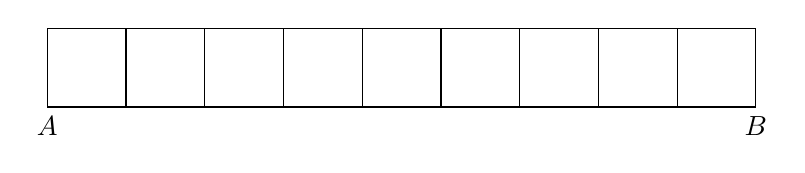
\begin{tikzpicture}
        \draw (0,0) node [below] {$A$} -- (9,0) node [below] {$B$};
        \draw (0,1) -- (9,1);
        \foreach \i in {0,1,...,9} {\draw (\i,0) -- (\i,1);};
    \end{tikzpicture}
\end{center}
\item 由$1$分, $2$分, $5$分, $1$角, $2$角, $5$角, $1$元, $2$元, $5$元, $10$元人民币各一张, 可组成多少种不同的币值?
\item 壹分币$3$枚、贰角币$6$张、拾元币$4$张, 可以组成多少种不同的币值?
\item 求$21600$的正约数的个数($1$和$21600$也是约数)及所有约数之和.
\item 设自然数$N=\{1,2,3,\cdots\}$的子集中含有$4$个元素的子集的个数记为$m$, 且这$m$个集合中所有元素之和为$\dfrac 1{12}\mathrm{P}_{100}^5$, 求$m$.
\item 有$11$名工人, 其中$5$名只会做钳工, $4$名只会做车工, $2$名既会做钳工, 又会做车工, 今要选$4$名车工、$4$名钳工, 有多少种不同的选法?
\item 设$(1+x+x^2)^n=a_0+a_1x+a_2x^2+\cdots +a_{2n}x^{2n}$, 求$a_0+a_2+a_4+\cdots +a_{2n}$的值.
\item 求$(\sqrt x+2)^{2n+1}$的展开式中$x$的整数次幂的各项系数之和.
\item 求$(1+i)^{4k-2}$($k\in \mathbf{N}$)展开式中奇数项之和.
\item 求证: $(3+\sqrt 7)^n$($n\in \mathbf{N}$, $n\ge 2$)的整数部分为奇数.


\end{enumerate}
\end{document}